\begin{appendices}
\section{Student Git}\label{Git}
\href{https://github.com/Lukas4314/SemesterProjekt-2}{https://github.com/Lukas4314/SemesterProjekt-2}
\section{Table of work distribution}\label{Work Distribution}
\begin{table}[H]
    \centering
    \begin{tabular}{c|c c c}
        Section & Main contributer & Supporting contributers \\
        \hline
        Vision & Lukas \\
        \hline
        Chessinterface & Karl \& Alexander & Lukas \\
        \hline
        Gripper & Nikolai \& Rasmus & Karl\\
        \hline
        Pico communication & Nikolai \& Rasmus & Lukas \& Magne \\
        \hline
        Electronics & Nikolai, Lukas \& Rasmus \\
        \hline
        Motionplanning & Magne\\
        \hline
    \end{tabular}
    \label{tab: work distribution}
\end{table}

\section{Sequence diagram}\label{fig: sequencediagram}
\begin{figure} [H]
    \centering
    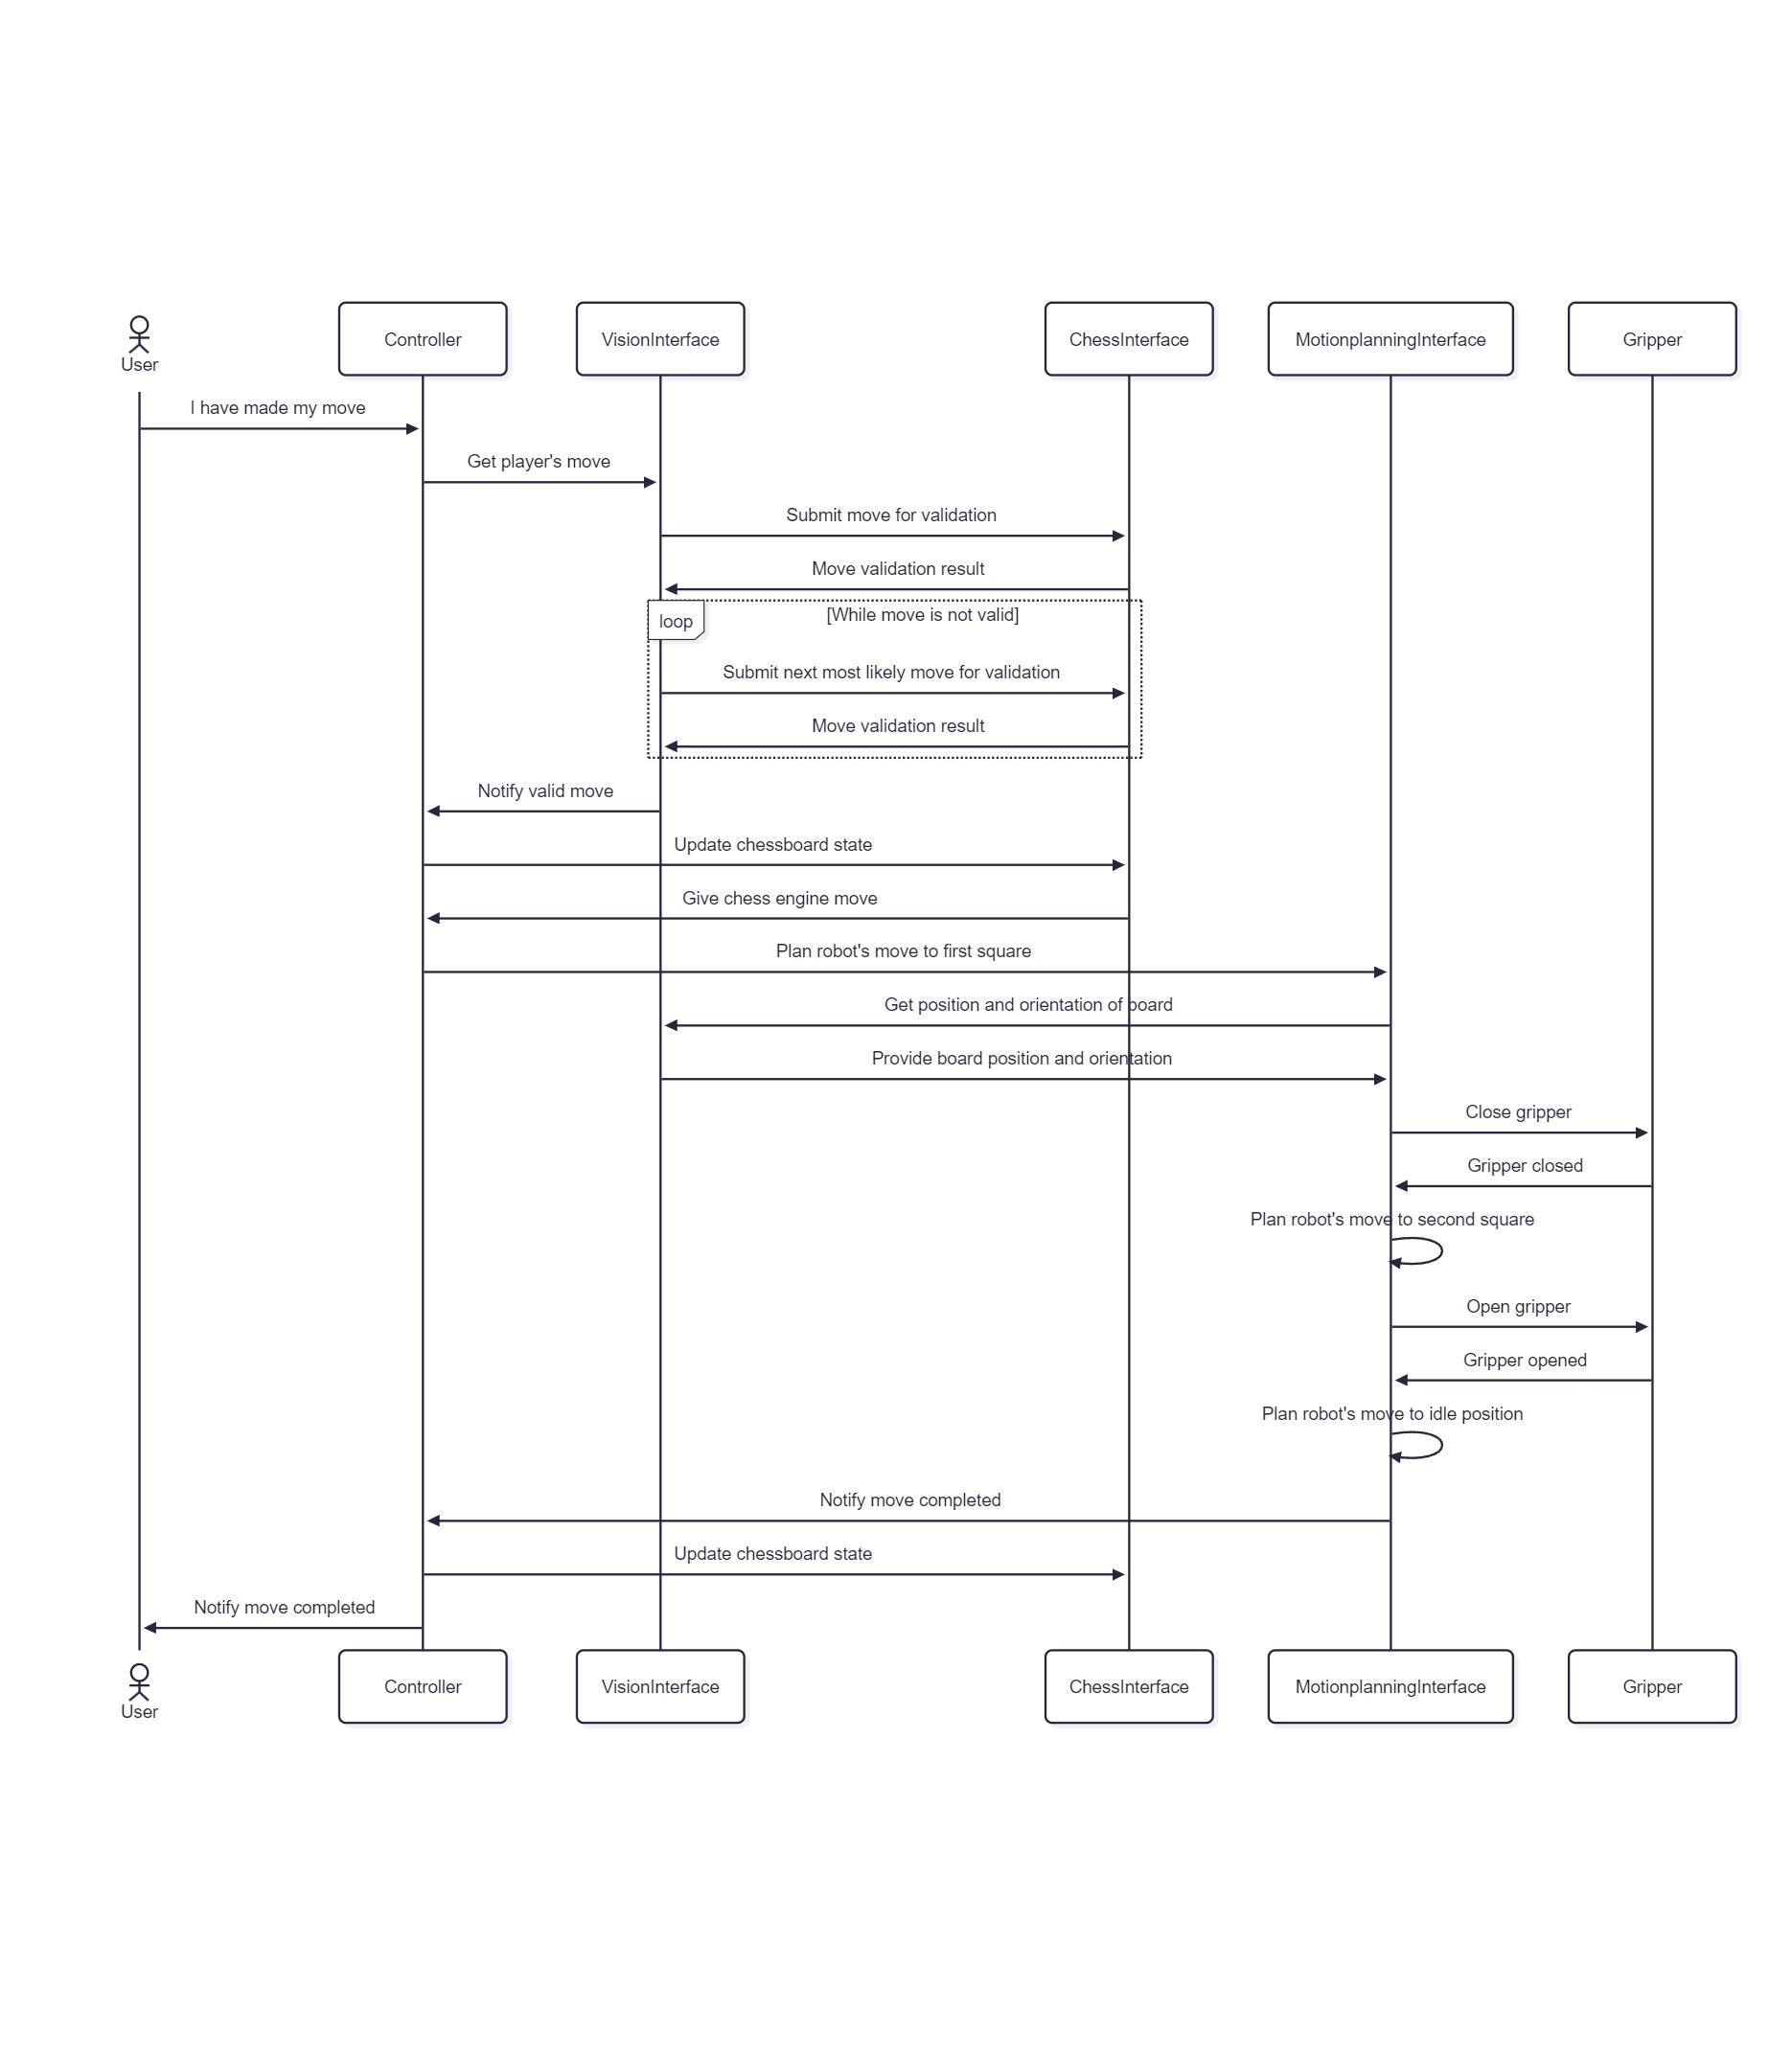
\includegraphics[width=1\linewidth]{Pictures/_plaintext_chess_robot_move_.png}
    \caption*{Sequence diagram of the execution of a regular move on the pc.}
\end{figure}

\section{Work drawings of the gripper} \label{Work_drawings_gripper}
Found in provided zip-file 
\section{Raw data from testing}\label{app:testdata}
Found in provided zip-file 
\section{Video of one test}\label{app:testvideo}
https://youtu.be/w2yRH1gf-pQ?si=PDSN-Km5NSTb24NZ

\end{appendices}